\documentclass[a4paper, 10pt]{article}

%--------------------------------------------------------------------------------
%% Packages

\usepackage[french]{babel}
\usepackage[T1]{fontenc}
\usepackage[utf8]{inputenc}

\usepackage{amssymb}
\usepackage{amsthm, thmtools}
\usepackage{amsmath}
\usepackage{amsfonts}
\usepackage{mathrsfs}
\usepackage{mathtools}
\usepackage{stmaryrd}
\usepackage{dsfont}
\usepackage[all]{xy}

\usepackage[top=1cm, bottom=1cm, left=1cm, right=1cm]{geometry}

%\usepackage{enumitem}

%\usepackage{nameref, hyperref, cleveref}
%	\hypersetup{
%		pdfnewwindow=false,
%		colorlinks=true,
%		linkcolor=black,
%		filecolor=black,
%		urlcolor=blue,
%		}

%\usepackage{multicol}
%	\setlength{\columnseprule}{0.1pt}

%\usepackage{titletoc}
%\usepackage{titlesec}
%	\titleformat{name = \chapter, numberless}[display]{\normalfont\Large\filcenter}{\vspace{-1cm}\titlerule[1pt]\vspace{1pt}\titlerule}{-0.5pc}{\LARGE\filcenter}[\vspace{1pc}\titlerule]
%	\titleformat{name = \chapter}[display]{\normalfont\Large\filcenter}{\vspace{-0.5cm}\titlerule[1pt]\vspace{1pt}\titlerule}{-0.5pc}{\Large\filcenter}[\vspace{0.5pc}\titlerule]
%	\titleformat{name = \section, numberless}[display]{\normalfont\Large\filcenter}{\vspace{-0.5cm}\titlerule[1pt]\vspace{1pt}\titlerule}{-0.5pc}{\Large\filcenter}[\vspace{0.5pc}\titlerule]
%	\titlespacing{\chapter}{0pt}{0pt}{*5}

%\allowdisplaybreaks
%\jot=0pt

%--------------------------------------------------------------------------------
%% Structures

\declaretheorem[numbered = yes, name = Definition, refname = {definition, definitions}, Refname = {Definition, Definitions}]{definition}
\declaretheorem[numbered = yes, name = Lemma, refname = {lemma, lemmas}, Refname = {Lemma, Lemmas}]{lemma}
\declaretheorem[numbered = yes, name = Theorem, refname = {theoreme, theorems}, Refname = {Theorem, Theorems}]{theorem}
\declaretheorem[numbered = yes, name = Proposition, refname = {proposition, propositions}, Refname = {Proposition, Propositions}]{proposition}
\declaretheorem[numbered = yes, name = Corollary, refname = {corollary, corollaries}, Refname = {Corollary, Corollaries}]{corollary}
\declaretheorem[numbered = yes, name = Example, refname = {example, examples}, Refname = {Example, Examples}]{example}
\declaretheorem[numbered = yes, name = Note, refname = {note, notes}, Refname = {Note, Notes}]{note}

%--------------------------------------------------------------------------------
%% Personal commands

%%% For probabilities & statistics
\renewcommand{\P}{\mathbb{P}}
\newcommand{\E}{\mathbb{E}}
\newcommand{\F}{\mathcal{F}}

%%% Usual sets
\newcommand{\R}{\mathbb{R}}
\newcommand{\N}{\mathbb{N}}
\newcommand{\Z}{\mathbb{Z}}
\newcommand{\Q}{\mathbb{Q}}

\newcommand{\Rd}{\mathbb{R}^{d}}
\newcommand{\Rn}{\mathbb{R}^{n}}
\newcommand{\Rp}{\mathbb{R}^{p}}
\newcommand{\Rq}{\mathbb{R}^{q}}

\renewcommand{\L}{L^{1}}
\newcommand{\Ld}{L^{2}}
\newcommand{\Lp}{L^{p}}
\newcommand{\Linf}{L^{\infty}}

\renewcommand{\l}{\ell^{1}}
\newcommand{\ld}{\ell^{2}}
\newcommand{\linf}{\ell^{\infty}}


%%% Specific 
\def\tf#1{\mathcal{F}\left(#1\right)}
\def\tfi#1{\overline{\mathcal{F}}\left(#1\right)}

\newcommand\independent{\protect\mathpalette{\protect\independenT}{\perp}}
\def\independenT#1#2{\mathrel{\rlap{$#1#2$}\mkern2mu{#1#2}}}

\newcommand{\drond}[2]{\frac{\partial #1}{\partial #2}}

%--------------------------------------------------------------------------------

\title{TP Supervised Learning Compte-rendu}
\author{Antoine Moulin}
\date{}

\begin{document}

\maketitle

\section{Emotion Recognition based on facial landmarks}

\begin{itemize}

	\item[1.] On importe les modules et fonctions nécessaires. \\
	
	\item[2.] Les données contiennent des visages ainsi que des points de repère associés à ces derniers. Pour chacun de ces exemples, on a la classe associée ("neutre" ou "joyeux"). \\
	
	\item[3.] On mélange les données afin que l'ensemble d'entraînement soit le plus représentatif possible du cas général. Par exemple, si notre ensemble d'entraînement est rangé par classe, il est nécessaire de mélanger celui-ci. \\
	
	\item[4.] On exécute la cellule permettant d'afficher les points alignés avec une GPA. \\
	
	\item[5.] On normalise les données afin que toutes les features aient le même ordre de grandeur. Cela permet notamment de donner la même importance à chaque feature. Après avoir utilisé une LDA, on obtient la matrice de confusion suivante :
	
\begin{center}
	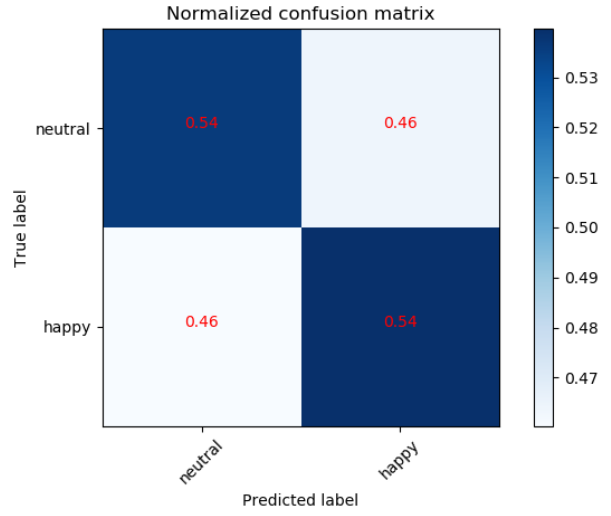
\includegraphics[scale=0.7]{confusion_matrix.PNG}
\end{center}
	
\hspace*{2mm}	
	
Les résultats ne sont pas très bons. En effet, en lisant la première ligne, on constate que parmi tous les visages dont l'expression est "neutre", seulement $54\%$ ont été classés comme "neutre". En lisant la première colonne, on remarque que sur tous les visages classés comme "neutre", seulement $54\%$ sont effectivement dans la classe "neutre". On pourrait faire de même avec la classe "joyeux". Ainsi, on peut dire que le classifieur se trompe "plus ou moins une fois sur deux". Cela vient sans doute du fait qu'en utilisant les distances au lieu des positions, on perd l'information spatiale (une distance par rapport à la moyenne peut correspondre à n'importe quel point situé sur le cercle ayant pour centre la moyenne et pour rayon cette même distance). \\
	
	\item[6.] On utilise directement les positions des points de repère comme features. Les résultats illustrés par la matrice de confusion semblent bien meilleurs : \\
	
\begin{center}
	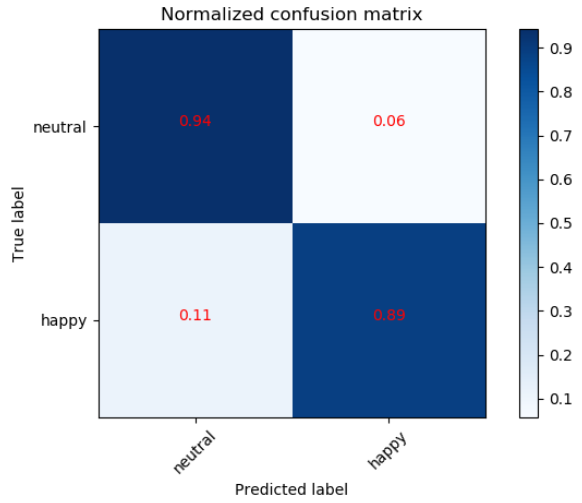
\includegraphics[scale=0.7]{confusion_matrix_positions.PNG}
\end{center}	
	
\hspace*{2mm}	
	
	\item[7.] La fonction \texttt{cross\_val\_score} appelle la fonction \texttt{score} du classifieur utilisé. Ainsi, dans chacune des méthodes (LDA, QDA, régression logistique ainsi que KNN), c'est la précision moyenne qui est renvoyée. Les résultats obtenus pour chaque méthode sont légèrement meilleurs que ceux obtenus à la question 5. Néanmoins, ils restent peu satisfaisants (de l'ordre de $0.6$) : \\
	
\begin{center}
	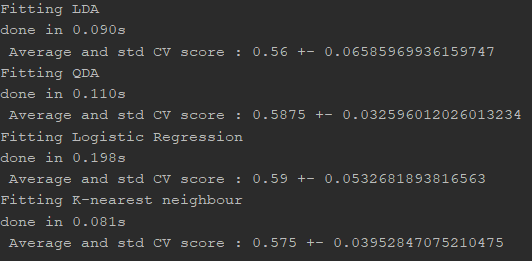
\includegraphics[scale=0.9]{scores.PNG}
\end{center}
	
\hspace*{2mm}
	
	\item[8.] Cette fois, les résultats sont bien meilleurs. Excepté pour la QDA qui obtient un score de $0.68$, les autres méthodes ont un score supérieur à $0.93$, soit un résultat similaire à celui obtenu à la question $6$. Nous obtenons effectivement des avertissements lors de l'utilisation d'une LDA ou d'une QDA : \\
	
\begin{center}
	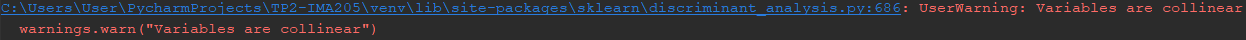
\includegraphics[scale=0.6]{discriminant_analysis_warning.PNG}
\end{center}
	
\hspace*{2mm}	
	
Le fait qu'on obtienne des avertissements vient du fait que certaines variables sont colinéaires. C'est problématique car si des variables sont (presque) colinéaires, alors le déterminant de la matrice de covariance est proche de $0$ et l'inversion de la matrice de covariance est peu précis. Le meilleur classifieur étant donné, dans le modèle LDA, par (cf cours) :

\[ f^{*}(x_{j}) = arg \, \min_{C_{k}} - 2 x_{j}^{T} \left( \Sigma^{*} \right)^{-1} \mu_{k}^{*} + \left( \mu_{k}^{*} \right)^{T} \left( \Sigma^{*} \right)^{-1} \mu_{k}^{*} - 2 log \left( \pi_{C_{k}}^{*} \right) \]

on remarque que le problème d'inversion de la matrice de covariance a un impact non négligeable sur notre classifieur. \\

	\item[9.] Dans le cadre d'une LDA, on suppose que les données suivent une distribution gaussienne. Il est donc possible d'utiliser une PCA. Dans notre cas, cela serait pertinent car la PCA nous fournit une base orthogonale, ce qui résout le problème de colinéarité. Les résultats obtenus sont globalement meilleurs. Si l'amélioration est faible pour ceux qui étaient déjà à $0.95$, la QDA fournit maintenant de bien meilleurs résultats, passant de $0.68$ à $0.95$. \\
	
	\item[10.] Nous pourrions choisir comme points de repère deux points situés aux extrémités gauche et droite de la bouche, ainsi qu'un troisième point situé au milieu de la lèvre supérieure car, a priori, une personne "joyeuse" sera en train de sourire tandis qu'une personne "neutre" ne sourira pas. Cela correspond par exemple aux points $0, 55, 61$. Nous pourrions également tenter de prendre les points qui maximisent la somme des variances selon l'axe des abscisses et l'axe des ordonnées. Dans les deux cas, voici ce que nous obtenons : \\

\begin{center}
	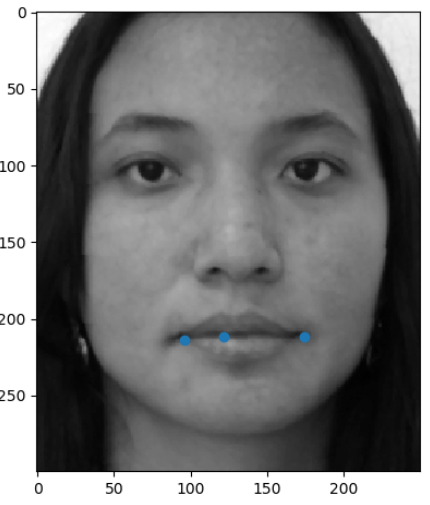
\includegraphics[scale=0.8]{mouth_points.PNG}
	\hspace*{1cm}
	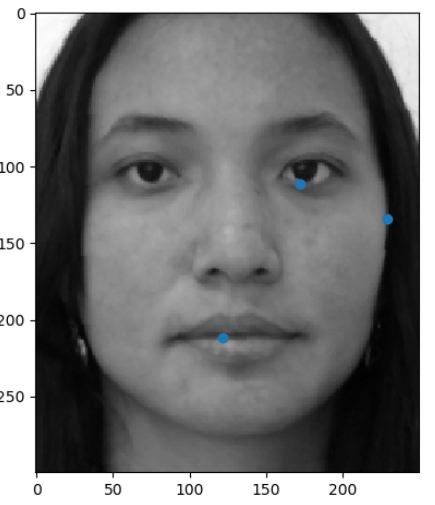
\includegraphics[scale=0.8]{max_var_points.PNG}
\end{center}

\vspace*{2mm}

Dans le second cas, nous obtenons un point situé sur la bouche, un en dessous d'un oeil et un autre à l'extrêmité d'une joue, ce qui est cohérent puisque ces parties du visage bougent de façon importante lorsqu'une personne sourit. \\

	\item[11.] Il est possible que les images n'aient pas été correctement annotées et donc qu'il y ait quelques erreurs dans la vérité terrain (même si elles doivent être peu nombreuses). Après tout, l'erreur est humaine ...

\end{itemize}

\section{Alzheimer prediction using PET signals}

On charge les données avec le code donné dans l'énoncé et on l'affiche : \\

\begin{center}
	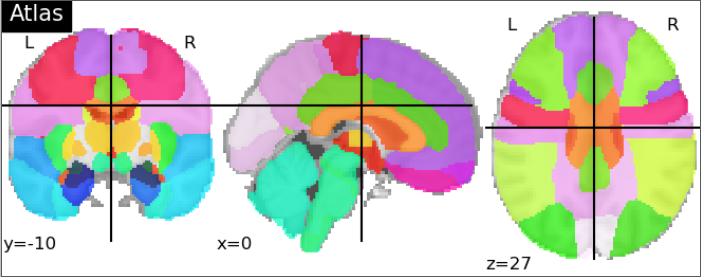
\includegraphics[scale=0.8]{ROIs.PNG}
\end{center}

On commence par implémenter le script \texttt{main\_ADNI.py} qui prédit si un patient est atteint de la maladie d'Alzheimer ou non. En utilisant une LDA comme dans la première partie, on obtient la matrice de confusion suivante : \\

\begin{center}
	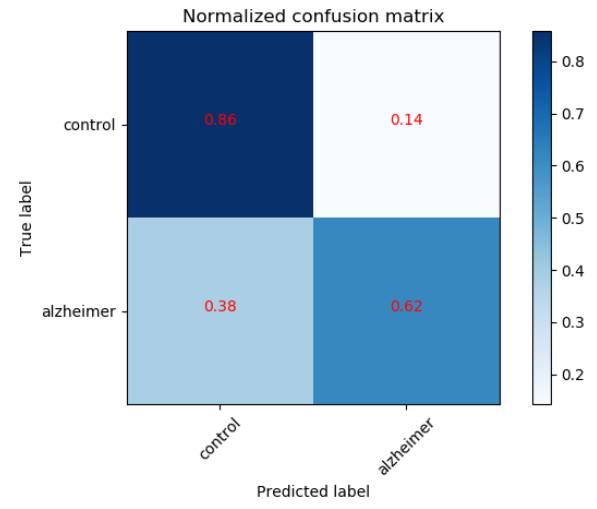
\includegraphics[scale=0.7]{confusion_matrix_alzheimer.PNG}
\end{center}

\hspace*{2mm}

\begin{itemize}

	\item[•] Si on utilise moins de sujets pour l'entraînement, on remarque que l'erreur d'entraînement a tendance à augmenter, tandis que l'erreur de test reste relativement élevée.
	
	\item[•] Il n'est pas nécessaire d'utiliser toutes les régions d'intérêts. On pourrait utiliser les régions mentionnées, à savoir l'hippocampe gauche, l'hippocampe droit, lobe temporal médian gauche et lobe temporal médian droit. On réalise ensuite une PCA sur ces quatre régions en gardant quatre composantes. Cela permet d'avoir une base orthonormée et donc de régler les problèmes de colinéarité. Pour sélectionner les régions, on utilise la variable \texttt{labels} qui est à notre disposition.
	
	\item[•] En essayant les différentes méthodes, on remarque que c'est la LDA qui donne de meilleurs résultats, avec un score de $0.87$.

\end{itemize}

\section{Theoretical questions}

	\subsection{OLS}

Avant de commencer les calculs, rappelons le contexte dans lequel nous nous plaçons dans cette partie. $\textbf{x}$ est une matrice réelle de taille $n \times d$ et $\textbf{y} \in \R^{n}$ est défini par : \[ \textbf{y} = \textbf{x}\beta + \epsilon \,\, t.q. \,\, \left\{ \begin{array}{c}
\mathbb{E} \left( \epsilon \right) = 0 \\
Var \left( \epsilon \right) = \sigma^{2} I_{n} \end{array}\right. \]

L'inégalité portant sur des matrices symétriques (car $Var \left( \beta^{*} \right), Var \left( \tilde{\beta} \right) \in \R^{d \times d}$ sont symétriques), il faut également définir une relation d'ordre sur cet ensemble. Pour $V_{1}, V_{2} \in \R^{d \times d}$, on dira que $V_{1} \leq V_{2}$ si, pour tout $u \in \R^{d}$, $u^{T}V_{1}u \leq u^{T}V_{2}u$. \\

On définit maintenant deux estimateurs non biaisés de $\beta$ : l'estimateur des moindres carrés $\beta^{*} = \left( \textbf{x}^{T} \textbf{x} \right)^{-1}\textbf{x}^{T} \textbf{y} = H \textbf{y}$ et un estimateur linéaire $\tilde{\beta} = C \textbf{y} = \left( H + D \right) \textbf{y}$ avec $D$ une matrice non nulle. \\

\begin{itemize}

	\item[•] \underline{Calcul de $\E \left( \tilde{\beta} \right)$}. Comme $\tilde{\beta}$ est un estimateur non biaisé de $\beta$, on a $\E \left( \tilde{\beta} \right) = \beta$. Si on détaille le calcul, on a : 

\[ \begin{array}{ccc} 
\E \left( \tilde{\beta} \right) & = & \left( H + D \right) \E \left( \textbf{y} \right) \\
 & = & \left( H + D \right) \textbf{x} \beta \,\,\,\,\,\, \\
 & = & H\textbf{x}\beta + D\textbf{x}\beta \,\,\,\, \end{array} \]

Or $H = \left( \textbf{x}^{T} \textbf{x} \right)^{-1}\textbf{x}^{T}$ donc $H \textbf{x} = I_{d}$. De plus, comme $\tilde{\beta}$ est non biaisé, alors $\E \left( \tilde{\beta} \right) = \beta$ d'où 

\[ \beta + D \textbf{x} \beta = \beta \,\, i.e. \,\, D \textbf{x} \beta = 0 \]

Ceci étant valable pour tout $\beta$, on a $D \textbf{x} = 0$. Ainsi,

\[ \boxed{\E \left( \tilde{\beta} \right) = \beta \,\, et \,\, D \textbf{x} = 0} \]

	\item[•] \underline{Calcul de $Var \left( \tilde{\beta} \right)$}. On a :
	
\[ \begin{array}{ccc} 
Var \left( \tilde{\beta} \right) & = & Var \left[ \left( H + D \right) \textbf{y} \right] \,\,\,\,\,\,\,\,\,\,\,\,\,\,\,\,\,\,\,\,\,\,\,\,\,\,\,\,\,\,\,\,\,\,\,\,\,\,\,\,\,\,\,\,\,\,\,\,\,\,\,\,\,\,\,\,\,\,\,\,\,\,\,  \\
 & = & Var \left( H \textbf{y} \right) + Var \left( D \textbf{y} \right) + 2 Cov \left( H \textbf{y}, D \textbf{y} \right) \end{array} \]

De plus, $Cov \left( H \textbf{y}, D \textbf{y} \right) = Cov \left( H \epsilon, D \epsilon \right) = \E \left( H \epsilon \epsilon^{T} D^{T} \right) = H \E \left( \epsilon \epsilon^{T} \right) D^{T} = \sigma^{2}H D^{T}$. Or d'après ce qui précède, $D \textbf{x} = 0$ donc $x^{T} D^{T} = 0$ puis $H D^{T} = 0$. Ainsi, $Cov \left( H \textbf{y}, D \textbf{y} \right) = 0$. \\

\noindent Comme $Var \left( D \textbf{y} \right) = D Var \left( \textbf{y} \right) D^{T} = D Var \left( \epsilon \right) D^{T} = \sigma^{2} DD^{T}$, on a 

\[ Var \left( \tilde{\beta} \right) = Var \left( \beta^{*} \right) + \sigma^{2} DD^{T} \]

Or \[ Var \left( \beta^{*} \right) = Var \left( \left( \textbf{x}^{T}\textbf{x} \right)^{-1} \textbf{x}^{T} y \right) = \E \left( \left( \textbf{x}^{T}\textbf{x} \right)^{-1}\textbf{x}^{T} \epsilon \epsilon^{T} \textbf{x} \left( \textbf{x}^{T}\textbf{x} \right)^{-1} \right ) = \left( \textbf{x}^{T}\textbf{x} \right)^{-1}\textbf{x}^{T} \E \left( \epsilon \epsilon^{T} \right) \textbf{x} \left( \textbf{x}^{T}\textbf{x} \right)^{-1} = \sigma^{2} \left( \textbf{x}^{T}\textbf{x} \right)^{-1} \]

Donc \[ \boxed{Var \left( \tilde{\beta} \right) = \sigma^{2} \left( \textbf{x}^{T}\textbf{x} \right)^{-1} + \sigma^{2}DD^{T}} \]

	\item[•] \underline{Inégalité}. Soit $u \in \R^{d}$. Alors :

\[ u^{T} Var \left( \tilde{\beta} \right) u = u^{T} Var \left( \beta^{*} \right) u + \sigma^{2} u^{T}DD^{T}u = u^{T} Var \left( \beta^{*} \right) u + \sigma^{2} \left|\left| D^{T}u \right|\right|^{2} \geq u^{T} Var \left( \beta^{*} \right) u \] 

Il y a égalité si, et seulement si, $D$ est nulle. Or $D$ est par hypothèse non-nulle. On peut donc conclure :

\[ \boxed{Var \left( \tilde{\beta} \right) > Var \left( \beta^{*} \right)} \]

\end{itemize}
	
	\subsection{Ridge regression}
	
\begin{itemize}

	\item[•] On rappelle (cf cours) que l'estimateur Ridge est donné par \[ \beta_{ridge}^{*} = \left( \textbf{x}_{c}^{T}\textbf{x}_{c} + \lambda I_{d} \right)^{-1}\textbf{x}_{c}^{T}\textbf{y}_{c} \]

Calculons son espérance.

\[ \E \left( \beta_{ridge}^{*} \right) = \left( \textbf{x}_{c}^{T}\textbf{x}_{c} + \lambda I_{d} \right)^{-1}\textbf{x}_{c}^{T} \E \left( \textbf{y}_{c} \right) = \left( \textbf{x}_{c}^{T}\textbf{x}_{c} + \lambda I_{d} \right)^{-1}\textbf{x}_{c}^{T} \textbf{x}_{c} \beta = \left( \textbf{x}_{c}^{T}\textbf{x}_{c} + \lambda I_{d} \right)^{-1} \left( \textbf{x}_{c}^{T} \textbf{x}_{c} + \lambda I_{d} - \lambda I_{d} \right) \beta \]

Ainsi,

\[ \boxed{\E \left( \beta_{ridge}^{*} \right) - \beta = - \lambda \left( \textbf{x}_{c}^{T}\textbf{x}_{c} + \lambda I_{d} \right)^{-1} \beta \neq 0} \]

Donc \underline{$\beta_{ridge}^{*}$ est un estimateur biaisé de $\beta$}.

	\item[•] On reprend l'expression de l'estimateur énoncée à la question précédente : \[ \beta_{ridge}^{*} = \left( \textbf{x}_{c}^{T}\textbf{x}_{c} + \lambda I_{d} \right)^{-1}\textbf{x}_{c}^{T}\textbf{y}_{c} \]

On remplace $\textbf{x}_{c}$ par $UDV^{T}$ : \[ \beta_{ridge}^{*} = \left( \left( UDV^{T} \right)^{T}UDV^{T} + \lambda I_{d} \right)^{-1}\left( UDV^{T} \right)^{T}\textbf{y}_{c} \]

C'est-à-dire \[ \beta_{ridge}^{*} = \left( VD^{T}U^{T}UDV^{T} + \lambda I_{d} \right)^{-1} VD^{T}U^{T} \textbf{y}_{c} \]

On utilise le fait que $U$ est une matrice orthogonale et que $D$ est une matrice diagonale : \[ \beta_{ridge}^{*} = \left( VD^{2}V^{T} + \lambda I_{d} \right)^{-1} VDU^{T} \textbf{y}_{c} \]

Comme $ \lambda I_{d} = \lambda VV^{T}$, on a : \[ \beta_{ridge}^{*} = \left( V \left( D^{2} + \lambda I_{d} \right)V^{T} \right)^{-1} VDU^{T} \textbf{y}_{c} \]

Puis \[ \boxed{\beta_{ridge}^{*} = V \left( D^{2} + \lambda I_{d} \right)^{-1} DU^{T} \textbf{y}_{c}} \]

Comme $D^{2} + \lambda I_{d}$ est une matrice diagonale, \underline{cette expression est utile car elle ne nécessite pas de calculer un inverse}, étant donné que l'inverse du matrice diagonale est la matrice diagonale formée des inverses des coefficients.

	\item[•] Calculons $Var \left( \beta_{ridge}^{*} \right)$ à l'aide de la décomposition en valeurs singulières. On utilise la formule de l'estimateur : 
	
\[ Var \left( \beta_{ridge}^{*} \right) = \sigma^{2} \left( \textbf{x}_{c}^{T}\textbf{x}_{c} + \lambda I_{d} \right)^{-1} \textbf{x}_{c}^{T}\textbf{x}_{c} \left( \textbf{x}_{c}^{T}\textbf{x}_{c} + \lambda I_{d} \right)^{-1} \]

$\textbf{x}_{c}^{T}\textbf{x}_{c}$ est une matrice symétrique donc d'après le théorème spectral, on peut écrire $\textbf{x}_{c}^{T}\textbf{x}_{c} = Q \Delta Q^{T}$ avec $\Delta$ une matrice diagonale et $Q$ une matrice orthogonale. Ainsi, on peut écrire :

\[ \textbf{x}_{c}^{T}\textbf{x}_{c} \left( \textbf{x}_{c}^{T}\textbf{x}_{c} + \lambda I_{d} \right)^{-1} = Q \Delta Q^{T} \left( Q \left( \Delta + \lambda I_{d} \right) Q^{T} \right)^{-1} = Q \Delta \left( \Delta + \lambda I_{d} \right)^{-1} Q^{T} \]

Or les matrices $\Delta$ et $\left( \Delta + \lambda I_{d} \right)^{-1}$ étant diagonales, elles commutent. Ainsi,

\[ \textbf{x}_{c}^{T}\textbf{x}_{c} \left( \textbf{x}_{c}^{T}\textbf{x}_{c} + \lambda I_{d} \right)^{-1} = Q \left( \Delta + \lambda I_{d} \right)^{-1} \Delta Q^{T} = \left( \textbf{x}_{c}^{T}\textbf{x}_{c} + \lambda I_{d} \right)^{-1} \textbf{x}_{c}^{T}\textbf{x}_{c} \]

On a donc, pour la variance, 

\[ Var \left( \beta_{ridge}^{*} \right) = \sigma^{2} \left( \textbf{x}_{c}^{T}\textbf{x}_{c} + \lambda I_{d} \right)^{-2} \textbf{x}_{c}^{T}\textbf{x}_{c} \]

On utilise la décomposition en valeurs singulières de $\textbf{x}_{c}$ :

\[ Var \left( \beta_{ridge}^{*} \right) = \sigma^{2} V \left( D^{2} + \lambda I_{d} \right)^{-2} D^{2}V^{T} \]

On a donc :

\[ Var \left( \beta_{ridge}^{*} \right) = \sigma^{2} \sum_{k = 1}^{d} \frac{s_{k}^{2}}{\left( s_{k}^{2} + \lambda \right)^{2}} v_{i}v_{i}^{T} \]

où $\left( s_{k} \right)_{k \in [\![ 1, d ]\!]}$ sont les valeurs singulières de $\textbf{x}_{c}$. D'où 

\[ Var \left( \beta_{ridge}^{*} \right) = \sigma^{2} \sum_{k = 1}^{d} \frac{\lambda_{k}}{\left( \lambda_{k} + \lambda \right)^{2}} v_{i}v_{i}^{T} \]

où les $\left( \lambda_{k} \right)_{k \in [\![ 1, d ]\!]}$ sont les valeurs propres de $\textbf{x}_{c}$. Or, de la même façon, on trouve : 

\[ Var \left( \beta_{OLS}^{*} \right) = \sigma^{2} \sum_{k = 1}^{d} \frac{1}{\lambda_{k}} v_{i}v_{i}^{T} \]

Comme, pour tout $k$, on a $\frac{\lambda_{k}}{\left( \lambda_{k} + \lambda \right)^{2}} < \frac{1}{\lambda_{k}}$, on peut conclure :

\[  \boxed{Var \left( \beta_{OLS}^{*} \right) \geq Var \left( \beta_{ridge}^{*} \right)} \]

	\item[•] D'après la formule précédente de la variance, on a clairement 
	
\[ \boxed{Var \left( \beta_{ridge}^{*} \right) \underset{\lambda \longrightarrow + \infty}{\longrightarrow} 0} \]

De plus, l'espérance tend vers $0$ lorsque $\lambda$ tend vers $+ \infty$, donc \[ \boxed{\E \left( \beta_{ridge}^{*} \right) - \beta \underset{\lambda \longrightarrow + \infty}{\longrightarrow} - \beta} \]

	\item[•] On reprend l'expression donné plus haut. On remplace $\textbf{x}_{c}^{T}\textbf{x}_{c}$ par $I_{d}$, on trouve $\beta_{ridge}^{*} = \frac{1}{1 + \lambda}\textbf{x}_{c}^{T}\textbf{y}_{c}$. Par ailleurs, on a également $\beta_{OLS}^{*} = \textbf{x}_{c}^{T}\textbf{y}_{c}$. D'où
	
\[ \boxed{\beta_{ridge}^{*} = \frac{1}{1 + \lambda} \beta_{OLS}^{*}} \]

	\item[•] On utilise le résultat précédent :

\[ \lambda \left( \frac{||\beta_{OLS}^{*}||_{2}^{2}}{(1 + \lambda)^{2}} - t \right) = 0 \]

\underline{Lorsque $\lambda = 0$}, on a \[ \boxed{\beta_{ridge}^{*} = \beta_{OLS}^{*}} \] 

et il n'y a pas de relation entre $\lambda$ et $t$ puisque dans ce cas, il n'y a pas de régularisation. \\

Supposons $\lambda \neq 0$. L'équation précédente donne \[ || \beta_{ridge}^{*} ||^{2} = \frac{\|\beta_{OLS}^*\|^2}{(1 + \lambda)^2} = t \] 

\underline{Lorsque $\lambda \longrightarrow + \infty$}, on a donc \[ \boxed{\beta_{ridge}^{*} = 0} \]

	\item[•] La régularisation Ridge a pour effet de forcer les coefficients à être dans une boule de rayon $\sqrt{t}$ mais sans forcément en mettre certains à $0$ tandis que la régularisation a pour propriété de mettre des coefficients à $0$ (ceux qui sont inférieurs en valeur absolue à $\frac{\lambda}{2}$).

\end{itemize}	
	
	\subsection{Elastic Net}

On peut se référer au cours de SD204 pour cette partie.
	
	\subsection{LDA}

\begin{itemize}

	\item[•] D'après le cours, nous avons \[ f^{*}(x_{j}) = \underset{C_{k}}{\operatorname{argmax}} \, P_{k}(X) \pi_{C_{k}} \]

\[ f^{*}(x_{j}) = \underset{C_{k}}{\operatorname{argmin}} \, -2 \log \left[ P_{k}(X)\pi_{C_{k}} \right] \]

De plus, à une constante près, nous avons

\[ P_{k}(X) = |\Sigma_{k}|^{- \frac{1}{2}} \exp \left( - \frac{1}{2} \left( x - \mu_{k} \right)^{T} \Sigma_{k}^{-1} \left( x - \mu_{k} \right) \right) \]

D'où

\[ f^{*}(x_{j}) = \underset{C_k}{\operatorname{argmin}} \, \left( x_{j} - \mu_{k} \right)^{T} \Sigma_{k}^{-1} \left( x_{j} - \mu_{k} \right) + \log | \Sigma_{k} | - 2 \log \left( \pi_{C_{k}} \right) \]

Puis

\[ f^{*}(x_{j}) = \underset{C_k}{\operatorname{argmin}} \, x_{j}^{T} \Sigma_{k}^{-1}x_{j} - x_{j}^{T} \Sigma_{k}^{-1} \mu_{k} - \mu_{k}^{T} \Sigma_{k}^{-1} x_{j}  + \mu_{k}^{T}  \Sigma_{k}^{-1} \mu_{k} - 2 \log \left( \pi_{C_{k}} \right) +  \log | \Sigma_{k} | \]

Finalement,

\[ \boxed{f^{*}(x_{j}) = \underset{C_k}{\operatorname{argmin}} \, x_{j}^{T} \Sigma_{k}^{-1} x_{j} - 2 x_{j}^{T} \Sigma_{k}^{-1} \mu_{k} - 2 \log \left( \pi_{C_{k}} \right) + \log | \Sigma_{k} |+ \mu_{k}^{T} \Sigma_{k}^{-1} \mu_{k}} \]

	\item[•] La solution est donc bien une \underline{fonction quadratique}, à cause du terme $x_{j}^{T} \Sigma_{k}^{-1} x_{j}$.


\end{itemize}

\end{document}